%!TEX root = ./binder.tex
%-------------------------------------------------------------------------------
\section{Introduction}
\label{sec:introduction}
%-------------------------------------------------------------------------------

Code coverage analysis is commonly used throughout the software testing process~\cite{Ammann2016}.
Structural coverage metrics such as statement and branch coverage can inspire confidence in a program under test (PUT), or at least identify untested code~\cite{Inozemtseva2014,Gopinath2014}.
Additionally, coverage analysis has demonstrated its usefulness in test suite reduction~\cite{Yoo2010}, fault localization~\cite{Pearson2017}, and detection of compiler bugs~\cite{Le2014}.
Moreover, certain coverage requirements are mandated by the standards in safety-critical domains~\cite{DO178C,ISO26262:2018}.

In recent years, feedback-guided fuzzing has emerged as a successful method for automatically discovering software bugs and security vulnerabilities~\cite{VUzzerRawat2017,kAFL:Schumilo2017,QSYMYun2018,Bohme2016a}. 
Notably, AFL~\cite{ZalewskiAFLWhitePaper} has pioneered the usage of code overage as a generic and effective feedback signal.
This success inspired a fuzzing ``renaissance'' and helped move fuzzing to  industrial-scale adoption like in Google's \mbox{OSS-Fuzz}~\cite{OSSFUZZ}.

In this work, we introduce {\bcov}, a tool for binary-level coverage analysis using static instrumentation.
{\bcov} works directly on x86-64 binaries in the ELF format without compiler support. 
It implements a trampoline-based approach where it inserts \textit{probes} in targeted locations to track \textit{basic block} coverage. 
Each probe consists of a \textit{detour} that diverts control flow to a designated \textit{trampoline}. 
The latter updates coverage data using a single pc-relative \texttt{mov} instruction, potentially executes relocated instructions, and then restores control flow to its original state.
Making this scheme to work efficiently and transparently on large and well-tested C and C++ programs required addressing several challenges:

\textbf{Probe pruning}~(\S\ref{sec:probe-pruning}). 
Instrumenting all basic blocks (BBs) can be inefficient, or even impossible, in x86-64 ISA due to its instruction-size variability.
We adopt the probe pruning technique proposed by Agrawal~\cite{Agrawal1994} where dominator relationships between BBs are used to group them in superblocks (SBs).
SBs are  arranged in a superblock dominator graph.
Covering a single BB implies that all BBs in the same SB are also covered, in addition to SBs dominating the current SB.
This allows us to significantly reduce the instrumentation overhead and size of coverage data.

\textbf{Precise CFG analysis}~(\S\ref{sec:controlflow}). 
Imprecision in the recovered control flow graph (CFG) can cause false positives in the reported coverage. 
It can also cause instrumentation errors which lead to crashes in a PUT.
To address this challenge, we propose \textit{sliced microexecution}, a precise and robust technique for jump table analysis. 
Also, we implement a non-return analysis that eliminates spurious CFG edges after non-return calls.
Our experiments show that {\bcov} can outperform IDA Pro, the leading industry disassembler.

\textbf{Static instrumentation}~(\S\ref{sec:instrumentation}). 
Given a set of BBs in an SB, we need to choose the best BB to probe based on the expected overhead of restoring control flow. 
We make this choice using a classification of BBs in \mbox{x86-64} into 9 types.
Also, some BBs can be too short to insert a detour. Their size is less than 5 bytes. 
We address this challenge by (1) aggressively exploiting padding bytes, (2) instrumenting jump table entries, and (3) introducing a greedy strategy for \textit{detour hosting} where a larger BB can host the detour of a neighboring short BB.
Combining these techniques with probe pruning enables tracking coverage of virtually all BBs.

\subsection{Design Overview}

% clip, left, bottom, right, top
\begin{figure}[t!]
    \centering
    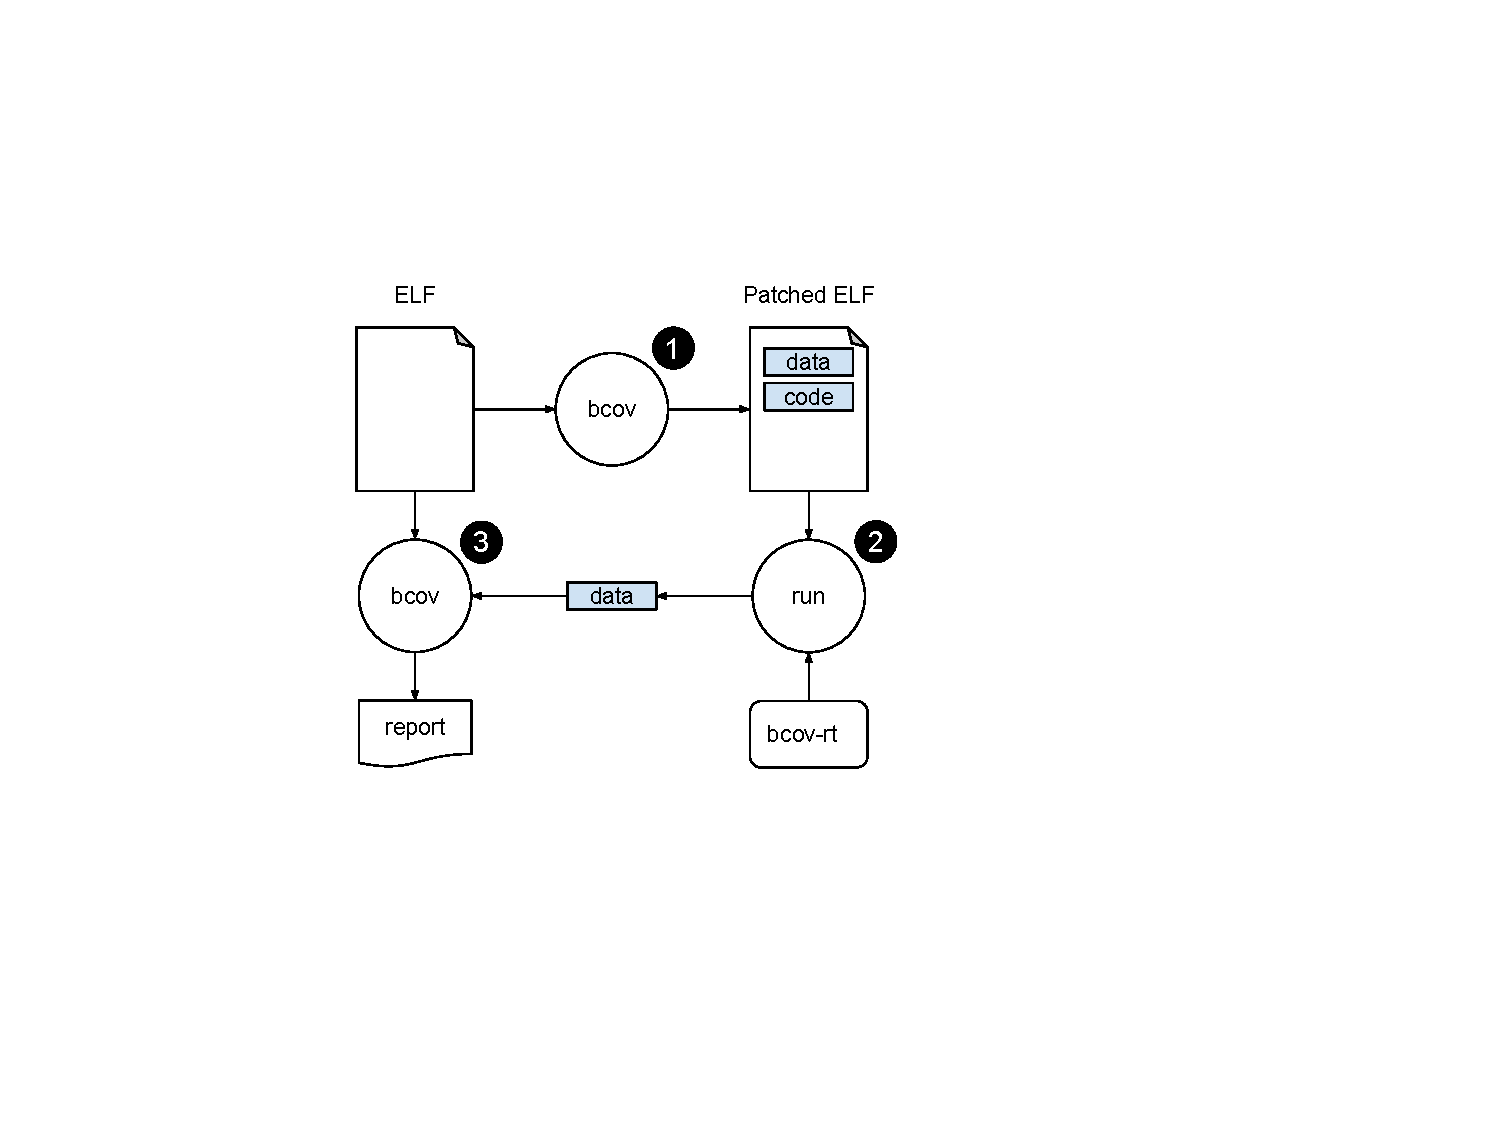
\includegraphics[clip, trim=5cm 5.8cm 10cm 4.8cm, width=0.35\textwidth]{fig/bcov-01-work-flow}
    \caption[workflow]{The general workflow of {\bcov}. 
        A binary is patched with extra code segment (trampolines) and data segment (coverage data). 
        Our \mbox{\textsf{bcov-rt}} library dumps the data segment at run-time. 
        In our prototype, reporting coverage requires re-analyzing the binary.}
    \Description{The general workflow of bcov}
    \label{fig:bcov-work-flow}
\end{figure}

Figure~\ref{fig:bcov-work-flow} depicts the workflow of {\bcov}.
Given an ELF module as input, {\bcov} first analyzes module-level artifacts, such as the call graph, before moving to function-level analyses to build the CFG and dominator graphs.
%Symbol information are used to identify functions. 
%In stripped binaries, {\bcov} can alternatively use call frame information which are generally available in the \texttt{.eh\_frame} section.
Then, {\bcov} will choose appropriate probe locations and estimate the required code and data sizes depending on the \textit{instrumentation policy} chosen by the user.
Our prototype supports two instrumentation policies.
The first is a \textit{complete} coverage policy where for \textit{any} test input it is possible to precisely identify covered BBs. 
The second one is a \textit{heuristic} coverage policy where we probe only the leaf SBs in the superblock dominator graph.
Running a test suite that covers \textit{all} leaf SBs implies that 100\% code coverage is reached. 
We refer to these policies as \textit{any-node} and \textit{leaf-node} policies respectively.
On average, the any-node policy probes 46\% of BBs compared to 30\% in the leaf-node policy.
Average performance overheads are 14\% and 8\% respectively.



The patching phase can start after completing the previous analysis phase.
Here, {\bcov} first extends the ELF module by allocating two loadable segments: a code segment where trampolines are written and a data segment for storing coverage data.
Then, {\bcov} iterates over all probes identified by the chosen instrumentation policy.
Each probe represents a single SB. 
Generally, patching a probe requires inserting a detour targeting its corresponding trampoline.
The detour can be a pc-relative \texttt{jmp} or \texttt{call} instruction.
The trampoline first updates coverage data and then restores control flow to its state in the original module as depicted in Figure~\ref{fig:patch-example}.

The data segment has a simple format consisting of a small header and a byte array that is initialized to zeros. 
Setting a byte to one indicates that its corresponding SB is covered. 
It is trivial to compress this data on disk as only the LSB of each byte is used.
For example, this enables storing complete coverage data of \texttt{llc} (LLVM backend) in 65KB only.~\footnote{The binary has around $1\times10^6$ BBs which contain more than $4\times10^6$ instructions.}
Our data format also enables merging coverage data of multiple tests using a simple bitwise OR operation.

Dumping coverage data requires linking against \textsf{bcov-rt}, our small runtime library.
Alternatively, \textsf{bcov-rt} can be injected using the 
{\allcap{LD\_PRELOAD} mechanism to avoid modifying the build system. 
Coverage data can be dumped on process shutdown or upon receiving a user signal.
The latter enables \textit{online} coverage tracking of long-running processes. 
Note that the data segment starts with a magic number which allows \textsf{bcov-rt} to identify it.

% clip, left, bottom, right, top
\begin{figure}[t!]
\centering
\vspace{-4pt}    
\begin{subfigure}[t]{0.23\textwidth}
	\begin{lstlisting}[style=custom-x64]
36b62: cmp  eax,0x140
36b67: sete al
36b6a: jmp  36bce
	\end{lstlisting}
	\vspace{-3pt}
	\caption{original code}
	\label{fig:2:original}
\end{subfigure}
\hfill
\begin{subfigure}[t]{0.23\textwidth}
	\begin{lstlisting}[style=custom-x64]
36b62: cmp  eax,0x140
36b67: jmp  6002b8
|
	\end{lstlisting}
	\vspace{-3pt}
	\caption{patched code}
	\label{fig:2:patch}
\end{subfigure}
\hfill
\begin{subfigure}[t]{0.38\textwidth}
	\vspace{-3pt}     
	\begin{lstlisting}[style=custom-x64]
6002b8: mov  BYTE PTR [rip+0xadd88],1
6002bf: sete al
6002c2: jmp  0x36bce
	\end{lstlisting}
	\vspace{-2pt}
	\caption{trampoline}
	\label{fig:2:trampoline}
\end{subfigure}

\caption{{\bcov} patching example. 
	(a) instruction at \textsf{0x36b67} must be relocated as the size of jump at \textsf{0x36b6a} is only two bytes. 
	(b)~relocated instructions are replaced with a 5 byte detour at \textsf{0x36b67}. 
	(c)~coverage update happens at \textsf{0x6002b8}. 
	Control flow is then restored after executing the relocated instruction at \textsf{0x6002bf}.}
    \Description{bcov patching example}
	\label{fig:patch-example}
\end{figure}

This design makes \textsf{bcov} achieve three main goals, namely, transparency, performance, and flexibility.
Program transparency is achieved by not modifying program stack, heap, nor any general-purpose register. 
Also, coverage update requires a single pc-relative \texttt{mov} instruction which has a modest performance overhead.
Finally, \textsf{bcov} works directly on the binary without compiler support and largely without changes to the build system. 
This enables users to flexibly adapt their instrumentation policy without recompilation.


%\subsection{Contributions}

To summarize, we make the following key contributions:
\begin{itemize}
    \item We are the first to bring Agrawal's probe pruning technique to binary-level instrumentation.
    We show that its superblocks can be effectively leveraged to optimize probe selection and reduce coverage data.
    
    \item We introduce \textit{sliced microexecution}, a robust method for jump table analysis.
    It significantly improves CFG precision and allows us to instrument jump table entries.
    
    \item We significantly push the state of the art in trampoline-based static instrumentation and show that it can be used to track code coverage efficiently and transparently.
         
\end{itemize}

We implemented our contributions in the tool \textsf{bcov}, which we make publicly available: 
\url{https://doi.org/10.5281/zenodo.3876047}
%\url{https://github.com/abenkhadra/bcov}.



We extensively experimented with \bcov. 
In this respect, we selected 8 popular and well-tested subjects such as \texttt{ffmpeg} and \texttt{llc}.
We compiled them using 4 recent major versions of \textsf{gcc} and \textsf{clang} at 3 different optimization levels each.
In total, we used \textsf{bcov} to instrument 95 binaries and more than 1.6 million functions.
Instrumented binaries did not introduce any test regressions.

%%% Local Variables:
%%% mode: latex
%%% TeX-master: "binder"
%%% End:
